\documentclass[11pt,a4paper]{article}
\usepackage[a4paper, total={7in, 10.25in}]{geometry}


\usepackage{color}
\usepackage{graphicx}
\usepackage{wrapfig}
\usepackage{fancyhdr}
\usepackage{tocloft}
\usepackage{multicol}
\usepackage{hyperref}
\usepackage{tabularx}
\usepackage{array}
\usepackage[export]{adjustbox}
\usepackage{listings}
\usepackage{xcolor}
    \definecolor{codegreen}{rgb}{0,0.6,0}
    \definecolor{codegray}{rgb}{0.5,0.5,0.5}
    \definecolor{codepurple}{rgb}{0.58,0,0.82}
    \definecolor{backcolour}{rgb}{1,1,1}

    \lstdefinestyle{mystyle}{
        backgroundcolor=\color{backcolour},   
        commentstyle=\color{codegreen},
        keywordstyle=\color{magenta},
        numberstyle=\tiny\color{codegray},
        stringstyle=\color{codepurple},
        basicstyle=\ttfamily\footnotesize,
        breakatwhitespace=false,         
        breaklines=true,                 
        captionpos=b,                    
        keepspaces=false,                 
        numbers=left,                    
        numbersep=5pt,                  
        showspaces=false,                
        showstringspaces=false,
        showtabs=false,                  
        tabsize=2
    }



\renewcommand{\cftsecleader}{\cftdotfill{\cftdotsep}}
\graphicspath{ {./images/} }
\hypersetup{
    colorlinks=true,
    linkcolor=blue,
    citecolor=black,
    filecolor=magenta,      
    urlcolor=cyan,
    pdftitle={Overleaf Example},
    pdfpagemode=FullScreen,
    }
\pagestyle{fancy}
\setlength{\headheight}{18pt}
\fancyhead[L]{\textit{EN3150 Pattern Recognition : Assignment 02}}
\fancyfoot[L]{\textit{Department of Electronic and Telecommunication \\University of Moratuwa}}

\title{DEPARTMENT OF ELECTRONIC AND TELECOMMUNICATION
UNIVERSITY OF MORATUWA

\vspace{10pt}

{\large{\textsc{EN 3150: Pattern recognition}}}

{\textsf{This is offered as a "EN 3150: Pattern Recognition" module's partial completion.}}

\vspace{30pt}

\includegraphics[scale=1.20]{images/University_of_Moratuwa_logo.png}

{\textsf{\textbf{Assignment 02 : Learning from data and related
challenges and classification.}}}}


\author{200686J : Vishagar A.}

\date{$2^{nd}$ of October, 2023}

\begin{document}

\maketitle

\newpage

\begin{abstract}
    \textit{This report deals with the explanation of the solutions for the given questions in the assignment 01 of the EN3150 module. The solutions are explained in a way that it is easy to understand and follow. The solutions are explained with the help of the code snippets and the results.We are mainly focussed on the learning from data and related challenges and classification.}    
\end{abstract}    

\vspace{50pt}
\tableofcontents


\newpage

\twocolumn

\section{Logistic Regression \& Weight Updating.}

In this section the code was given to generate data and we are supposed to implement the Batch Gradient Descent and Newton's Method to find the optimal weights for the given data. The data was generated using the following code.

\lstset{style=mystyle}
\lstinputlisting[language=Octave]{code1.py}

\subsection{Batch Gradient Descent}

And after the data was generated we are supposed to implement the Batch Gradient Descent we used the following equation.

\begin{equation}
    w_{t+1} \leftarrow w_{t} - \frac{\alpha}{N} \cdot( \mathbf{1}^T{diag}({sigm}(\mathbf{w}^T(t) \mathbf{x}_i) - y_i) \mathbf{X})^T
\end{equation}

\newpage

and the implementation of the above equation and the results are shown below.

\lstset{style=mystyle}
\lstinputlisting[language=Octave]{code2.py}



{\begin{figure}[h]
    \centering
    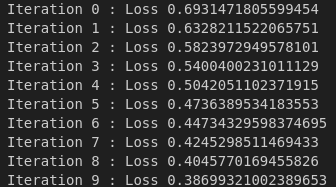
\includegraphics[width=1.0\linewidth]{images/1.png}
    \caption{Loss funstions after BGD}
\end{figure}}

\lstset{style=mystyle}
\lstinputlisting[language=Octave]{code3.py}

{\begin{figure}[h]
    \centering
    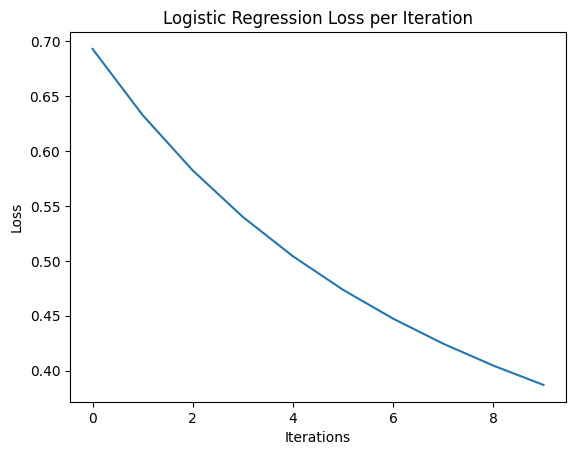
\includegraphics[width=0.95\linewidth]{images/12.png}
    \caption{Loss vs Iterations}
\end{figure}}

\newpage

\subsection{Newton's Method}

And after the data was generated we are supposed to implement the Newton's Method we used the following equation.

\begin{equation}
    w_{t+1} \leftarrow w_{t} - \frac{\alpha}{N} \cdot( \mathbf{1}^T{diag}({sigm}(\mathbf{w}^T(t) \mathbf{x}_i) - y_i) \mathbf{X})^T
\end{equation}

\begin{equation}
    {\alpha} = \frac{1}{N}\cdot \mathbf{X}^T \mathbf{S} \mathbf{X}
\end{equation}

\lstset{style=mystyle}
\lstinputlisting[language=Octave]{code4.py}

{\begin{figure}[h]
    \centering
    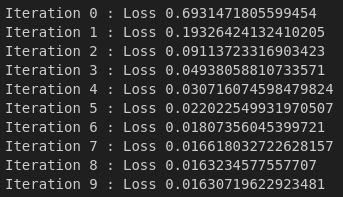
\includegraphics[width=1.0\linewidth]{images/2.png}
    \caption{Loss functions after Newton's Method}
\end{figure}}

\lstset{style=mystyle}
\lstinputlisting[language=Octave]{code5.py}

\newpage

{\begin{figure}[h]
    \centering
    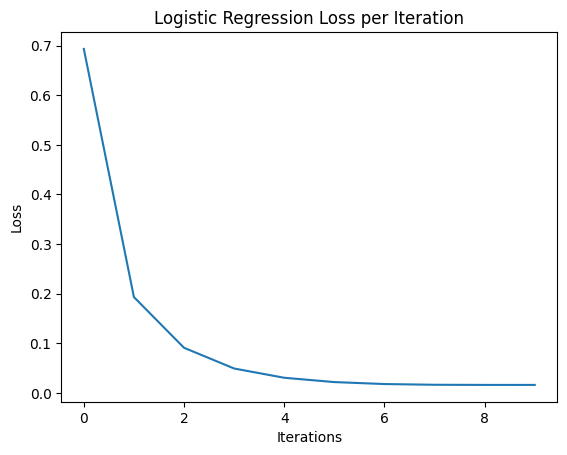
\includegraphics[width=1.0\linewidth]{images/22.png}
    \caption{Loss vs Iterations}
\end{figure}}

\subsection{Comparison between the two methods}

\begin{itemize}
    \item In the Newton's method the learnig rate changes with the iteration and in the Batch Gradient Descent the learning rate is constant.
    \item The Newton's method converges to the optimal value faster than the Batch Gradient Descent.
\end{itemize}

{\begin{figure}[h]
    \centering
    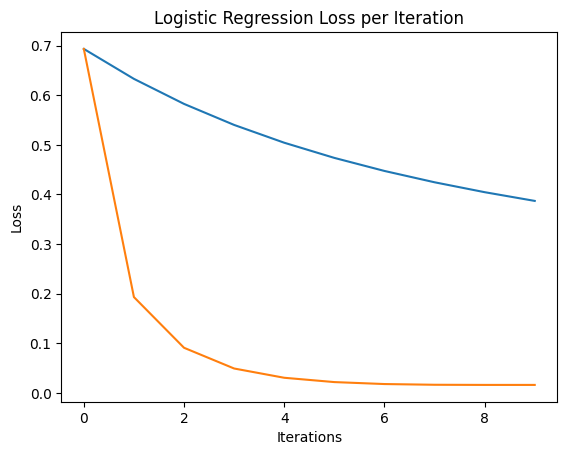
\includegraphics[width=1.0\linewidth]{images/3.png}
    \caption{Comparison of the two methods}
\end{figure}}

\newpage

\section {Grid search for hyperparameter tuning}
In this section we are supposed to perform a logistic regression for image classification, create a pipeline, define a parameter grid for hyper parameter tuning and perform a grid search for the hyper parameter tuning. The code for the above mentioned tasks are shown below.

\lstset{style=mystyle}
\lstinputlisting[language=Octave]{code6.py}

\subsection{Usage of Permutation}

In this section we used the permutation to generate random indices to generate new order of the data by shuffling the data rows randomly.\\\\
We used this permutation function for both X and Y where we can ensure that we will get a new order of the data for both X and Y.\\\\
And also we used this permutation to avoid order based bias in the data which could lead us to poor generalization of the model.

\subsection{Usage of Pipeline and GridSearch}

Here we were supposed to use lasso logistic regression for image classification and create a pipeline that includes the
scaling and the Lasso logistic regression estimator.\\\\

And then we were asked to define a parameter grid for hyper parameter tuning and perform a grid search for the hyper parameter tuning. we selected 9 equally spaced values staring from 0.01 to 100. (-2,2 in log scale)\\\\ 

We used the following code to create the pipeline.

\lstset{style=mystyle}
\lstinputlisting[language=Octave]{code7.py}

And got the best value for and the releated test accuracy as,

\begin{itemize}
    \item Best value for C : 0.31622776601683794
    \item Test accuracy : 0.85
\end{itemize}



\begin{figure}[h]
    \centering
    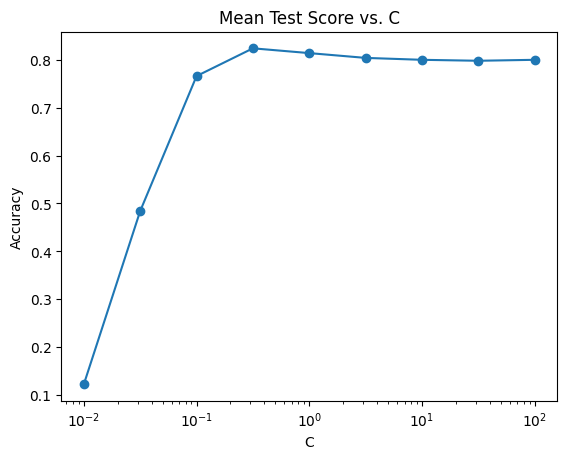
\includegraphics[width=1.0\linewidth]{images/4.png}
    \caption{Mean test score vs C}
\end{figure}

\newpage

And for the evaluation metrics we used \textbf{Precision}, \textbf{Recall}, \textbf{confusion matrix} and \textbf{F1 score} and following were the relevant codes and results.

\lstset{style=mystyle}
\lstinputlisting[language=Octave]{code8.py}

\begin{figure}[h]
    \centering
    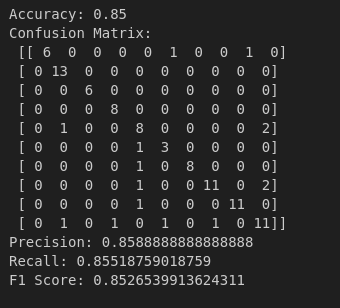
\includegraphics[width=1.0\linewidth]{images/5.png}
    \caption{Evaluation metrics}
\end{figure}

\newpage

\begin{figure}
    \centering
    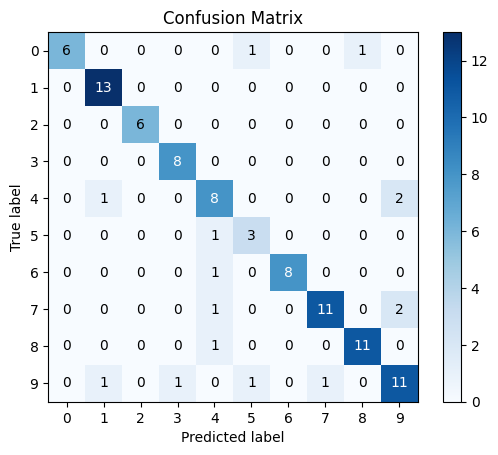
\includegraphics[width=1.0\linewidth]{images/52.png}
    \caption{Confusion matrix}
\end{figure}

Considering the above results we can say that the model is performing well and the model is not overfitting or underfitting. Because the \textbf{accuracy of the model is high} and the \textbf{precision, recall and the F1 score are also high}. And also the \textbf{confusion matrix} shows that the model is performing well by only predicting the correct classes.

\section{Logistic Regression}

\begin{itemize}
    \item $x_{1}$ = Number of Hours studied
    \item $x_{2}$ = Student's GPA 
    \item y = 1 if the student Got $A^{+}$ and 0 otherwise
    \item $w_{0}$ = -6
    \item $w_{1}$ = 0.05
    \item $w_{2}$ = 1
\end{itemize}

The Regression model,

\begin{equation}
    Pr(y) = \frac{1}{1 + e^{-(w_{0} + w_{1}x_{1} + w_{2}x_{2})}}
\end{equation}

therefore, 

\newpage

\subsection{Answer for (a)}

\begin{itemize}
    \item $x_{1}$ = 40
    \item $x_{2}$ = 3.5
\end{itemize}

\begin{equation}
    Pr(y) = \frac{1}{1 + e^{-(w_{0} + w_{1}x_{1} + w_{2}x_{2})}}
\end{equation}

\begin{equation}
    Pr(y) = \frac{1}{1 + e^{-(-6 + 0.05 \times 40 + 1 \times 3.5)}}
\end{equation}

\begin{equation}
    Pr(y) = \frac{1}{1 + e^{-(-6 + 2 + 3.5)}}
\end{equation}

\begin{equation}
    Pr(y) = \frac{1}{1 + e^{(0.5)}}
\end{equation}

\begin{equation}
    Pr(y) = \frac{1}{1 + 1.648721}
\end{equation}

\begin{equation}
    Pr(y) = 0.37754
\end{equation}


\subsection{Answer for (b)}

\begin{itemize}
    \item Pr(y) = 0.5
    \item $x_{2}$ = 3.5
\end{itemize}


\begin{equation}
    Pr(y) = \frac{1}{1 + e^{-(w_{0} + w_{1}x_{1} + w_{2}x_{2})}}
\end{equation}

\begin{equation}
    0.5 = \frac{1}{1 + e^{-(w_{0} + w_{1}x_{1} + w_{2}x_{2})}}
\end{equation}

\begin{equation}
    e^{-(w_{0} + w_{1}x_{1} + w_{2}x_{2})} = 1
\end{equation}

\begin{equation}
    w_{0} + w_{1}x_{1} + w_{2}x_{2} = 0
\end{equation}


\begin{equation}
    -6 + 0.05 \times x_{1} + 1 \times 3.5 = 0
\end{equation}


\begin{equation}
    x_{1} = 50
\end{equation}



\section{References}

\begin{itemize}
    \item \href{https://scikit-learn.org/stable/modules/generated/sklearn.linear_model.LinearRegression.html}{Sci-kit Learn Documentation on Logistic regression}
    \item \href{https://scikit-learn.org/stable/auto_examples/compose/plot_digits_pipe.html}{Pipelining}
    \item \href{https://scikit-learn.org/stable/modules/generated/sklearn.model_selection.GridSearchCV.html}{Grid Search}
    % \item \href{ }{Github/EN3160_Assignment_01}
   
\end{itemize}

\section{Github Repository}

Following is the link to my Github repository for this assignment.\\

\href{https://github.com/Vgr20/EN3150_Assignment_02.git}{Github/EN3150\_Assignment\_02}


\end{document}




%%%%%%%%%%%%%%%%%%%%%%%%%%%%%%%%%%%%%%%%%%%%%%%%%%%%%%%%%%%%%%%%%%%%%%%%%%%%%%%%%%%%%%%%%%%%%%%%%%%%%%%%%%%%%%%%%%%%%%%%%%%%%%%%%%%%%%%%%%%%%%%%%%%%%%%%%%%%%%%%%%%%%%%%%%

% {\begin{center}
% \begin{tabular}{ | m{1.85cm} | m{0.85cm}| m{0.85cm} | m{0.85cm} | m{0.85cm} | m{0.85cm} | } 
%  \hline
%  Objectives& Weight & Design 01 & Design 02 & Design 03 & Design 04 \\  
%  \hline\hline
%  Efficiency & 10 & 7 & 8 & 8 & 9 \\
%  \hline
%  Mobility & 10 & 7 & 9 & 8 & 8 \\
%  \hline
%  Easy Maintenance & 10 & 7 & 6 & 5 & 8 \\
%  \hline
%  Refilling accessibility & 5 & 3 & 3 & 2 & 4 \\
%  \hline
%  Durability & 5 & 2 & 3 & 3 & 2 \\
%  \hline
%  Manufacture cost & 5 & 3 & 3 & 2 & 3 \\
%  \hline
%  Overall Look & 5 & 2 & 3 & 5 & 2 \\
%  \hline
%  \hline
%  Total & 50 & 31 & 35 & 33 & 36 \\
%  \hline
 
% \end{tabular}
% \end{center}}

%%%%%%%%%%%%%%%%%%%%%%%%%%%%%%%%%%%%%%%%%%%%%%%%%%%%%%%%%%%%%%%%%%%%%%%%%%%%%%%%%%%%%%%%%%%%%%%%%%%%%%%%%%%%%%%%%%%%%%%%%%%%%%%%%%%%%%%%%%%%%%%%%%%%%%%%%%%%%%%%%%%%%%%%%%


% \begin{center}
% \begin{tabular}{ | m{2cm} | m{5cm}| m{2cm} | m{6cm} | } 

%  \hline
%  Part Name & Description & Supplier & Part Link\\  
%  \hline\hline
%  NE555P & 8-pin Precise timer & Texas Instruments & \href{https://www.lcsc.com/product-detail/Timers-Clock-Oscillators_Texas-Instruments-NE555P_C46749.html}{NE555p data sheet}\\
%  \hline
%  2N2222A & Generic npn transistor & Slkor & \href{https://www.lcsc.com/product-detail/Bipolar-Transistors-BJT_Slkor-SLKORMICRO-Elec-2N2222A_C5330385.html}{2N2222A data sheet}\\
%  \hline
%   LM7805 & Linear voltage Regulators & LRC & \href{https://www.lcsc.com/product-detail/Linear-Voltage-Regulators-LDO_LRC-LR7805_C2846986.html}{Lm7805 Data sheet}\\
%  \hline
%   HC sr501 & Passive IR sensor & HC & \href{https://www.lcsc.com/product-detail/Timers-Clock-Oscillators_Texas-Instruments-NE555P_C46749.html}{HC sr501 data sheet}\\
%  \hline
%   KNSCHA ZE11000UF & 1000uF Capacitor & KNSCHA & \href{https://www.lcsc.com/product-detail/Solid-Capacitors_KNSCHA-ZE11000UF35V119EC0014_C2992586.html}{Capacitor data sheet}\\
%  \hline
%   Resistors & Resistors with different values & Texas Instruments & \href{https://www.lcsc.com/search?q=resistors%20through%20hole}{Through hole resistors}\\
%  \hline
 
% \end{tabular}  
% \end{center}
%%%%%%%%%%%%%%%%%%%%%%%%%%%%%%%%%%%%%%%%%%%%%%%%%%%%%%%%%%%%%%%%%%%%%%%%%%%%%%%%%%%%%%%%%%%%%%%%%%%%%%%%%%%%%%%%%%%%%%%%%%%%%%%%%%%%%%%%%%%%%%%%%%%%%%%%%%%%%%%%%%%%%%%%%%